
%%%%%%%%%%%%%%%%%%%%%%%%%%%%%%%%%%%%%%%%%
% Programming/Coding Assignment
% LaTeX Template
%
% This template has been downloaded from:
% http://www.latextemplates.com
%
% Original author:
% Ted Pavlic (http://www.tedpavlic.com)
%
% Note:
% The \lipsum[#] commands throughout this template generate dummy text
% to fill the template out. These commands should all be removed when 
% writing assignment content.
%
% This template uses a Perl script as an example snippet of code, most other
% languages are also usable. Configure them in the "CODE INCLUSION 
% CONFIGURATION" section.
%
%%%%%%%%%%%%%%%%%%%%%%%%%%%%%%%%%%%%%%%%%

%----------------------------------------------------------------------------------------
%	PACKAGES AND OTHER DOCUMENT CONFIGURATIONS
%----------------------------------------------------------------------------------------



\documentclass{article}

\usepackage{fancyhdr} % Required for custom headers
\usepackage{lastpage} % Required to determine the last page for the footer
\usepackage{extramarks} % Required for headers and footers
\usepackage[usenames,dvipsnames]{color} % Required for custom colors
\usepackage{graphicx} % Required to insert images
\usepackage{listings} % Required for insertion of code
\usepackage{courier} % Required for the courier font
\usepackage{lipsum} % Used for inserting dummy 'Lorem ipsum' text into the template
\usepackage{setspace}
\usepackage{color}
\usepackage{comment}
\usepackage{caption}
\usepackage[T1]{fontenc}
\usepackage{hyperref}
\usepackage{natbib}
\usepackage{underscore}
\usepackage{subfigure}
\usepackage{fixltx2e}

\hypersetup{
    colorlinks=true,
    linkcolor=blue,
    filecolor=magenta,      
    urlcolor=cyan,
    breaklinks=true
}

\usepackage[]{algorithm2e}
\usepackage{pdfpages}
\usepackage{tikz}




%For python inclusion (http://widerin.org/blog/syntax-highlighting-for-python-scripts-in-latex-documents)
\definecolor{Code}{rgb}{0,0,0}
\definecolor{Decorators}{rgb}{0.5,0.5,0.5}
\definecolor{Numbers}{rgb}{0.5,0,0}
\definecolor{MatchingBrackets}{rgb}{0.25,0.5,0.5}
\definecolor{Keywords}{rgb}{0,0,1}
\definecolor{self}{rgb}{0,0,0}
\definecolor{Strings}{rgb}{0,0.63,0}
\definecolor{Comments}{rgb}{0,0.63,1}
\definecolor{Backquotes}{rgb}{0,0,0}
\definecolor{Classname}{rgb}{0,0,0}
\definecolor{FunctionName}{rgb}{0,0,0}
\definecolor{Operators}{rgb}{0,0,0}
\definecolor{Background}{rgb}{0.98,0.98,0.98}

% Margins
\topmargin=-0.45in
\evensidemargin=0in
\oddsidemargin=0in
\textwidth=6.5in
\textheight=9.0in
\headsep=0.25in

\linespread{1.1} % Line spacing

% Set up the header and footer
\pagestyle{fancy}
\lhead{\hmwkAuthorName} % Top left header
\chead{\hmwkClass\ (\hmwkClassInstructor\ \hmwkClassTime): \hmwkTitle} % Top center head
\chead{\hmwkClass\ (\hmwkClassInstructor): \hmwkTitle} % Top center head
\rhead{\firstxmark} % Top right header
\lfoot{\lastxmark} % Bottom left footer
\cfoot{} % Bottom center footer
\rfoot{Page\ \thepage\ of\ \protect\pageref{LastPage}} % Bottom right footer
\renewcommand\headrulewidth{0.4pt} % Size of the header rule
\renewcommand\footrulewidth{0.4pt} % Size of the footer rule

\setlength\parindent{0pt} % Removes all indentation from paragraphs

%----------------------------------------------------------------------------------------
%	CODE INCLUSION CONFIGURATION
%----------------------------------------------------------------------------------------

\definecolor{MyDarkGreen}{rgb}{0.0,0.4,0.0} % This is the color used for comments
\lstloadlanguages{Perl} % Load Perl syntax for listings, for a list of other languages supported see: ftp://ftp.tex.ac.uk/tex-archive/macros/latex/contrib/listings/listings.pdf
\lstset{language=Perl, % Use Perl in this example
        frame=single, % Single frame around code
        basicstyle=\small\ttfamily, % Use small true type font
        keywordstyle=[1]\color{Blue}\bf, % Perl functions bold and blue
        keywordstyle=[2]\color{Purple}, % Perl function arguments purple
        keywordstyle=[3]\color{Blue}\underbar, % Custom functions underlined and blue
        identifierstyle=, % Nothing special about identifiers                                         
        commentstyle=\usefont{T1}{pcr}{m}{sl}\color{MyDarkGreen}\small, % Comments small dark green courier font
        stringstyle=\color{Purple}, % Strings are purple
        showstringspaces=false, % Don't put marks in string spaces
        tabsize=5, % 5 spaces per tab
        %
        % Put standard Perl functions not included in the default language here
        morekeywords={rand},
        %
        % Put Perl function parameters here
        morekeywords=[2]{on, off, interp},
        %
        % Put user defined functions here
        morekeywords=[3]{test},
       	%
        morecomment=[l][\color{Blue}]{...}, % Line continuation (...) like blue comment
        numbers=left, % Line numbers on left
        firstnumber=1, % Line numbers start with line 1
        numberstyle=\tiny\color{Blue}, % Line numbers are blue and small
        stepnumber=5 % Line numbers go in steps of 5
}

% Creates a new command to include a perl script, the first parameter is the filename of the script (without .pl), the second parameter is the caption
\newcommand{\perlscript}[2]{
\begin{itemize}
\item[]\lstinputlisting[caption=#2,label=#1]{#1.pl}
\end{itemize}
}


%----------------------------------------------------------------------------------------
%	DOCUMENT STRUCTURE COMMANDS
%	Skip this unless you know what you're doing
%----------------------------------------------------------------------------------------

% Header and footer for when a page split occurs within a problem environment
\newcommand{\enterProblemHeader}[1]{
\nobreak\extramarks{#1}{#1 continued on next page\ldots}\nobreak
\nobreak\extramarks{#1 (continued)}{#1 continued on next page\ldots}\nobreak
}

% Header and footer for when a page split occurs between problem environments
\newcommand{\exitProblemHeader}[1]{
\nobreak\extramarks{#1 (continued)}{#1 continued on next page\ldots}\nobreak
\nobreak\extramarks{#1}{}\nobreak
}

\setcounter{secnumdepth}{0} % Removes default section numbers
\newcounter{homeworkProblemCounter} % Creates a counter to keep track of the number of problems

\newcommand{\homeworkProblemName}{}
\newenvironment{homeworkProblem}[1][Problem \arabic{homeworkProblemCounter}]{ % Makes a new environment called homeworkProblem which takes 1 argument (custom name) but the default is "Problem #"
\stepcounter{homeworkProblemCounter} % Increase counter for number of problems
\renewcommand{\homeworkProblemName}{#1} % Assign \homeworkProblemName the name of the problem
\section{\homeworkProblemName} % Make a section in the document with the custom problem count
\enterProblemHeader{\homeworkProblemName} % Header and footer within the environment
}{
\exitProblemHeader{\homeworkProblemName} % Header and footer after the environment
}

\newcommand{\problemAnswer}[1]{ % Defines the problem answer command with the content as the only argument
\noindent\framebox[\columnwidth][c]{\begin{minipage}{0.98\columnwidth}#1\end{minipage}} % Makes the box around the problem answer and puts the content inside
}

\newcommand{\homeworkSectionName}{}
\newenvironment{homeworkSection}[1]{ % New environment for sections within homework problems, takes 1 argument - the name of the section
\renewcommand{\homeworkSectionName}{#1} % Assign \homeworkSectionName to the name of the section from the environment argument
\subsection{\homeworkSectionName} % Make a subsection with the custom name of the subsection
\enterProblemHeader{\homeworkProblemName\ [\homeworkSectionName]} % Header and footer within the environment
}{
\enterProblemHeader{\homeworkProblemName} % Header and footer after the environment
}

%----------------------------------------------------------------------------------------
%	NAME AND CLASS SECTION
%----------------------------------------------------------------------------------------

\newcommand{\hmwkTitle}{Assignment\ \#4 } % Assignment title
%\newcommand{\hmwkDueDate}{Saturday,\ March\ 28\ 2019} % Due date
\newcommand{\hmwkClass}{Web Science} % Course/class
%\newcommand{\hmwkClassTime}{10:30am} % Class/lecture time
\newcommand{\hmwkClassInstructor}{Alexander Nwala} % Teacher/lecturer
\newcommand{\hmwkAuthorName}{Apurva Modi} % Your name

%----------------------------------------------------------------------------------------
%	TITLE PAGE
%----------------------------------------------------------------------------------------

\title{
\vspace{2in}
\textmd{\textbf{\hmwkClass:\ \hmwkTitle}}\\
%\normalsize\vspace{0.1in}\small{Due\ on\ \hmwkDueDate}\\
%\vspace{0.1in}\large{\textit{\hmwkClassInstructor\ \hmwkClassTime}}
\vspace{0.1in}\large{\textit{\hmwkClassInstructor}}
\vspace{3in}
}

\author{\textbf{\hmwkAuthorName}}
\date{Sunday, March 24, 2019} % Insert date here if you want it to appear below your name

%----------------------------------------------------------------------------------------

\begin{document}

\maketitle
\newpage



%----------------------------------------------------------------------------------------
%	TABLE OF CONTENTS
%----------------------------------------------------------------------------------------

%\setcounter{tocdepth}{1} % Uncomment this line if you don't want subsections listed in the ToC

\newpage
\tableofcontents
\newpage

%----------------------------------------------------------------------------------------
%	PROBLEM 1
%----------------------------------------------------------------------------------------

% To have just one problem per page, simply put a \clearpage after each problem

\begin{homeworkProblem}

We know the result of the Karate Club (Zachary, 1977) split. Prove or disprove that the result of split could have been predicted by the weighted graph of social interactions. \\ How well does the
mathematical model represent reality?  \\
Generously document your answer with all supporting equations, code, graphs, arguments, etc.\\

\textbf{Clues: }
\begin{enumerate}
\item\textbf{} To Draw original Karate club graph (two connected components) after split (Week 6 lecture, slide 98).
\item\textbf{} To Run multiple iterations of graph partioning algorithm (e.g., Girvan-Newman Algorithm) on experimental Karate club graph until the graph splits into two connected components.
\item\textbf{} To Compare the connected components of the experimental graph (in 2.) with the original connected components of the split Karate club graph (in 1.). Are they similar?
 \end{enumerate}
 

\textbf{Useful sources include:}
\begin{enumerate}
 \item\textbf{Original paper}
 
http://aris.ss.uci.edu/~lin/76.pdf
 \item\textbf{Week 6 Slides:}
 
https://docs.google.com/presentation/d/1ihf6N8bHgzM5VLAyHkmF_i5JGUBVpCSdsvYpk8XgHwo/
edit?usp=sharing
 \item\textbf{Slides:}
 
http://www-personal.umich.edu/~ladamic/courses/networks/si614w06/ppt/lecture18.ppt\\
http://clair.si.umich.edu/si767/papers/Week03/Community/CommunityDetection.pptx
 \item\textbf{Code and Data:}
 
https://networkx.github.io/documentation/networkx-1.10/reference/generated/networkx.generators.social.
karate_club_graph.html

https://networkx.github.io/documentation/networkx-1.9/examples/graph/karate_club.html

http://nbviewer.ipython.org/url/courses.cit.cornell.edu/info6010/resources/11notes.ipynb

http://stackoverflow.com/questions/9471906/what-are-the-differences-between-community-detection
-algorithms-in-igraph/9478989\#9478989

http://stackoverflow.com/questions/5822265/are-there-implementations-of-algorithms-for-community-
detection-in-graphs

http://konect.uni-koblenz.de/networks/ucidata-zachary

http://vlado.fmf.uni-lj.si/pub/networks/data/ucinet/ucidata.htm\#zachary

https://snap.stanford.edu/snappy/doc/reference/CommunityGirvanNewman.html

http://igraph.org/python/doc/igraph-pysrc.html\#Graph.community_edge_betweenness

 \end{enumerate}
 
 \newpage
 
%\problemAnswer{

 \textbf{SOLUTION :}\\
 I have followed the pages and slides presented as part of the problem.
  \begin{enumerate}
  \item\textbf{} Install "Netwokx" library to generate the \textbf{karateClub} graph as below :
  			\begin{verbatim}
				pip install networkx
			\end{verbatim}
					
\item\textbf{} Import the \textbf{networkx} library and generate the \textbf{karateClub} graph
  	        		\begin{verbatim}
				import networkx as nx
				graph = nx.karate_club_graph()
			\end{verbatim}
			
\item\textbf{} Implement the \textbf{Girvan-Newman} algorithm as
  	        		\begin{enumerate}
			\item\textbf{}while number of connected subgraphs < specified number of clusters and the number of edges in graph > 0:
			\item\textbf{}calculate edge betweenness for every edge in the graph
			\item\textbf{}remove edge(s) with highest betweenness
			\item\textbf{}recalculate connected components	
			\end{enumerate} 	
							      
 \end{enumerate}
 
%}
  
\begin{lstlisting}[language=Python, caption=karateClubGraph.py]

import networkx as nx
import numpy as np
import matplotlib.pyplot as plt

graph = nx.karate_club_graph()
edgeCount = graph.number_of_edges()
maximumClusterThreshold = 2
count = 0
clusterCount = nx.algorithms.number_connected_components(graph)

# Drawing the initial karateclub graph
nx.draw(graph, with_labels=True)
plt.show()

while (edgeCount > 0 and clusterCount < maximumClusterThreshold):
   betweennessDict = nx.algorithms.betweenness.edge_betweenness(graph)
   maximumBetweennessValue = np.max(list(betweennessDict.values()))
   edgeValue = ''
   
   for edge in betweennessDict:
      if betweennessDict[edge] == maximumBetweennessValue:
         edgeValue = edge
         
   print ('Removing Edges...',str(edgeValue[0])+"--->"+str(edgeValue[1]))     
   graph.remove_edge(edgeValue[0], edgeValue[1])

   # Drawing the sequential karateclub graph
   nx.draw(graph, with_labels=True)t
   plt.show()
   count = count + 1
   clusterCount = nx.algorithms.number_connected_components(graph)
   
print('Total flows to separation:',count)
\end{lstlisting}

The above code, will separate the karateClub graph in to two components in a total of \textbf{10} iterations.

\begin{figure}[h]
  \centering
    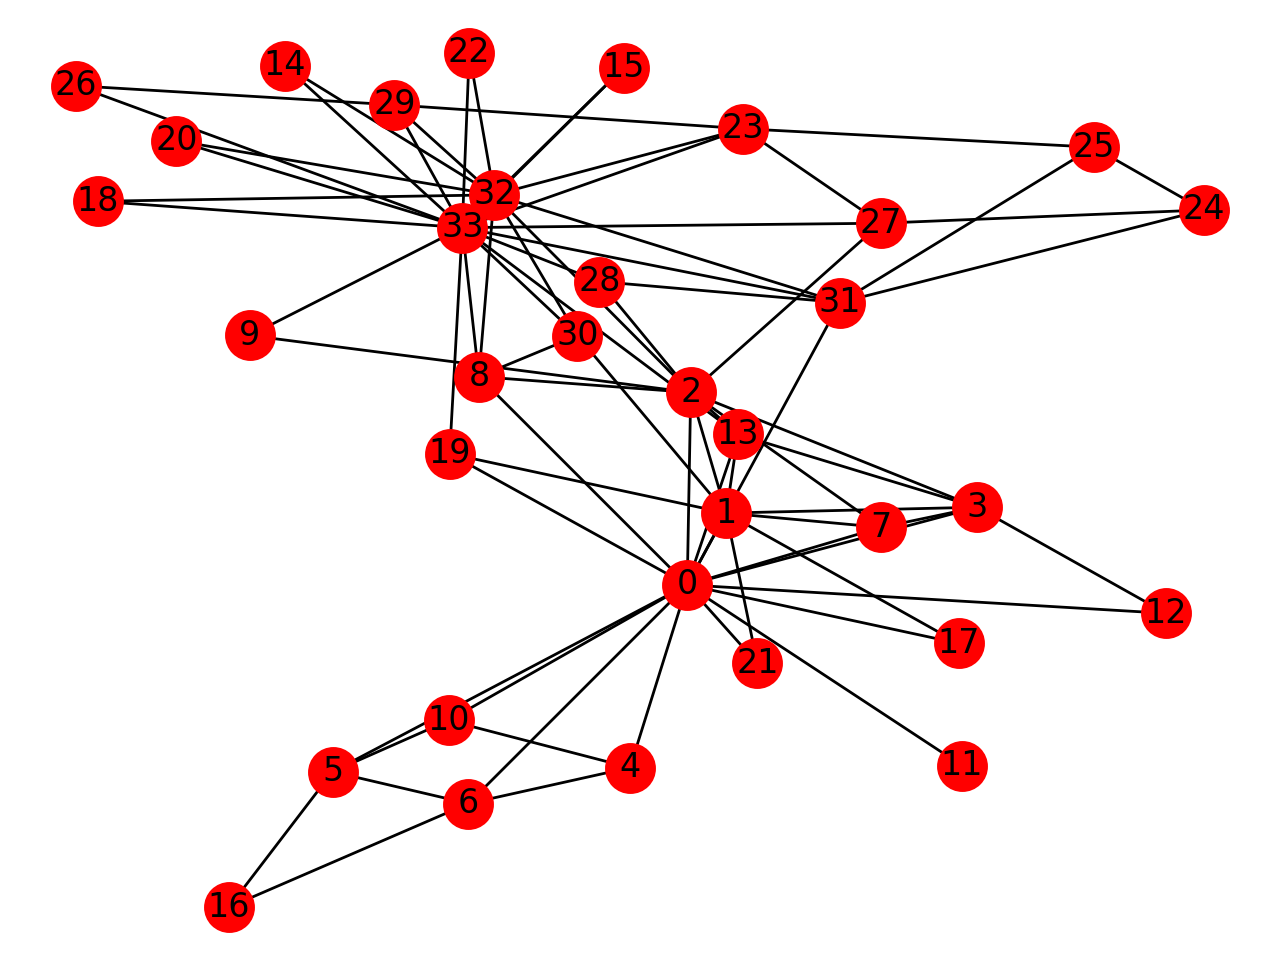
\includegraphics[width=0.8\textwidth]{F1}
      \caption{Original karate Club Graph}
	\end{figure}
	
\begin{figure}[h]
  \centering
    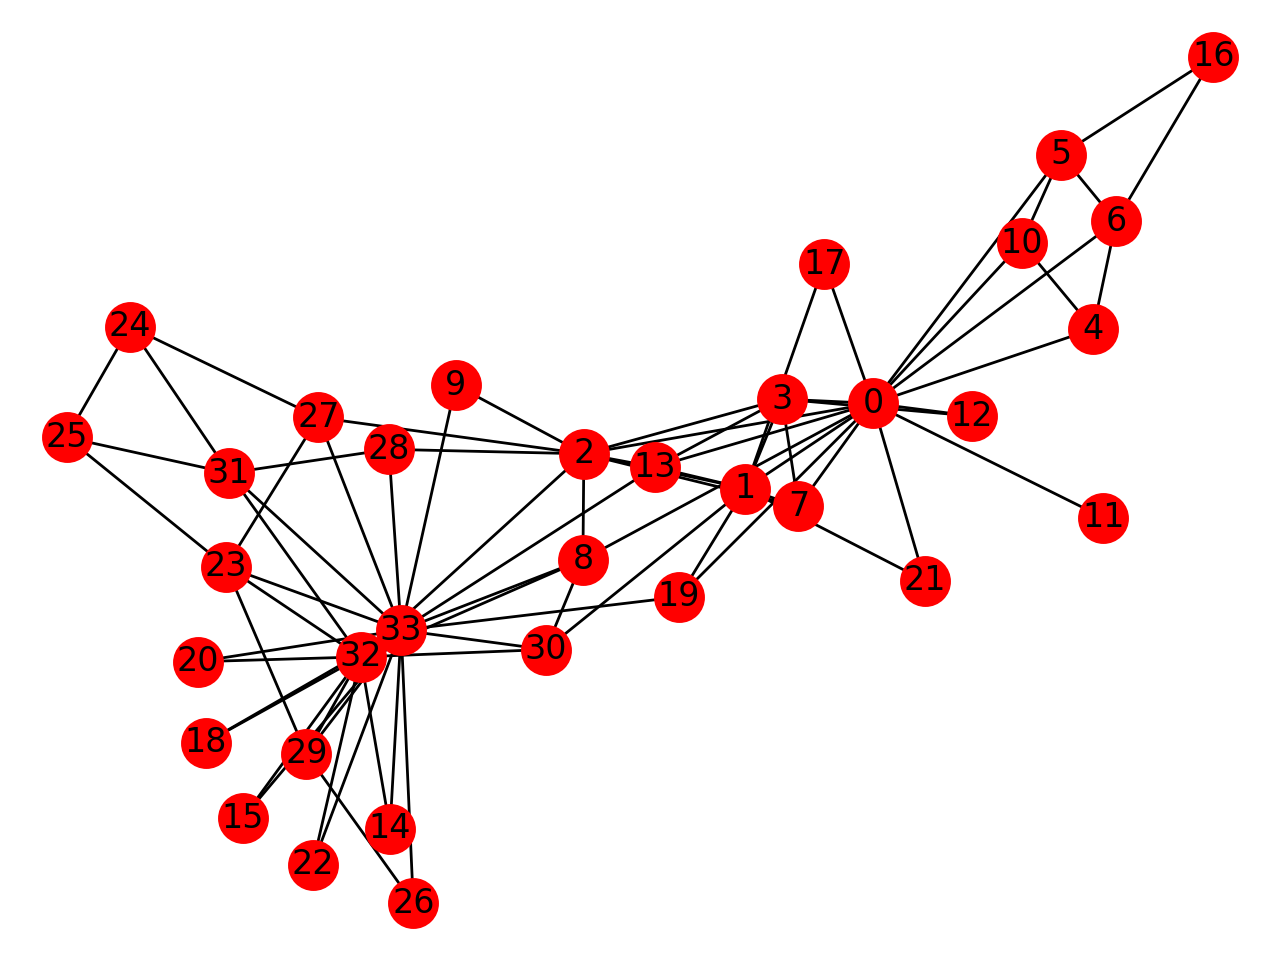
\includegraphics[width=0.8\textwidth]{F2}
      \caption{Iteration 1}
	\end{figure}
	
\begin{figure}[h]
  \centering
    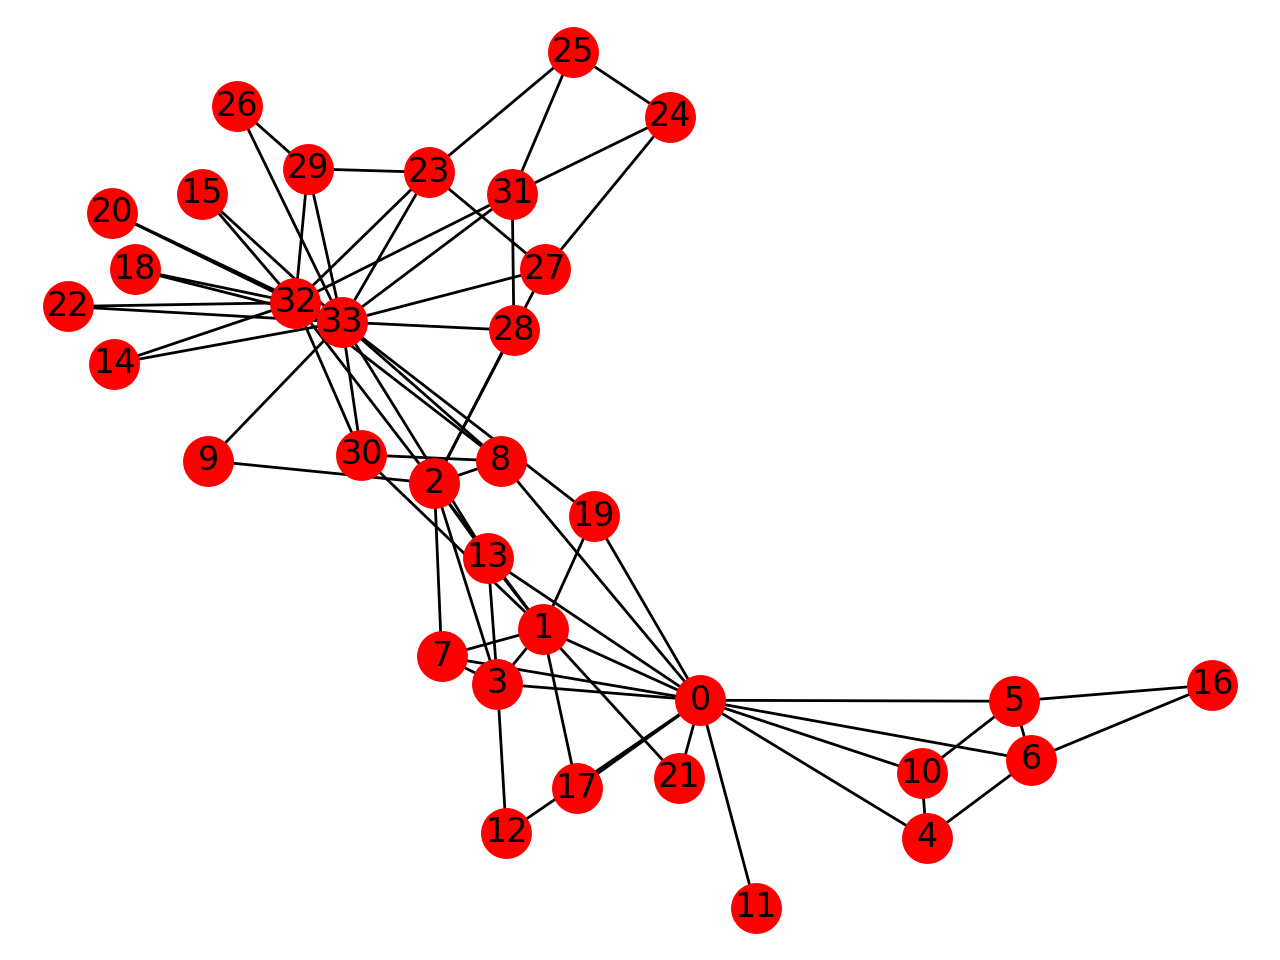
\includegraphics[width=0.8\textwidth]{F3}
      \caption{Iteration 2}
	\end{figure}
	
\begin{figure}[h]
  \centering
    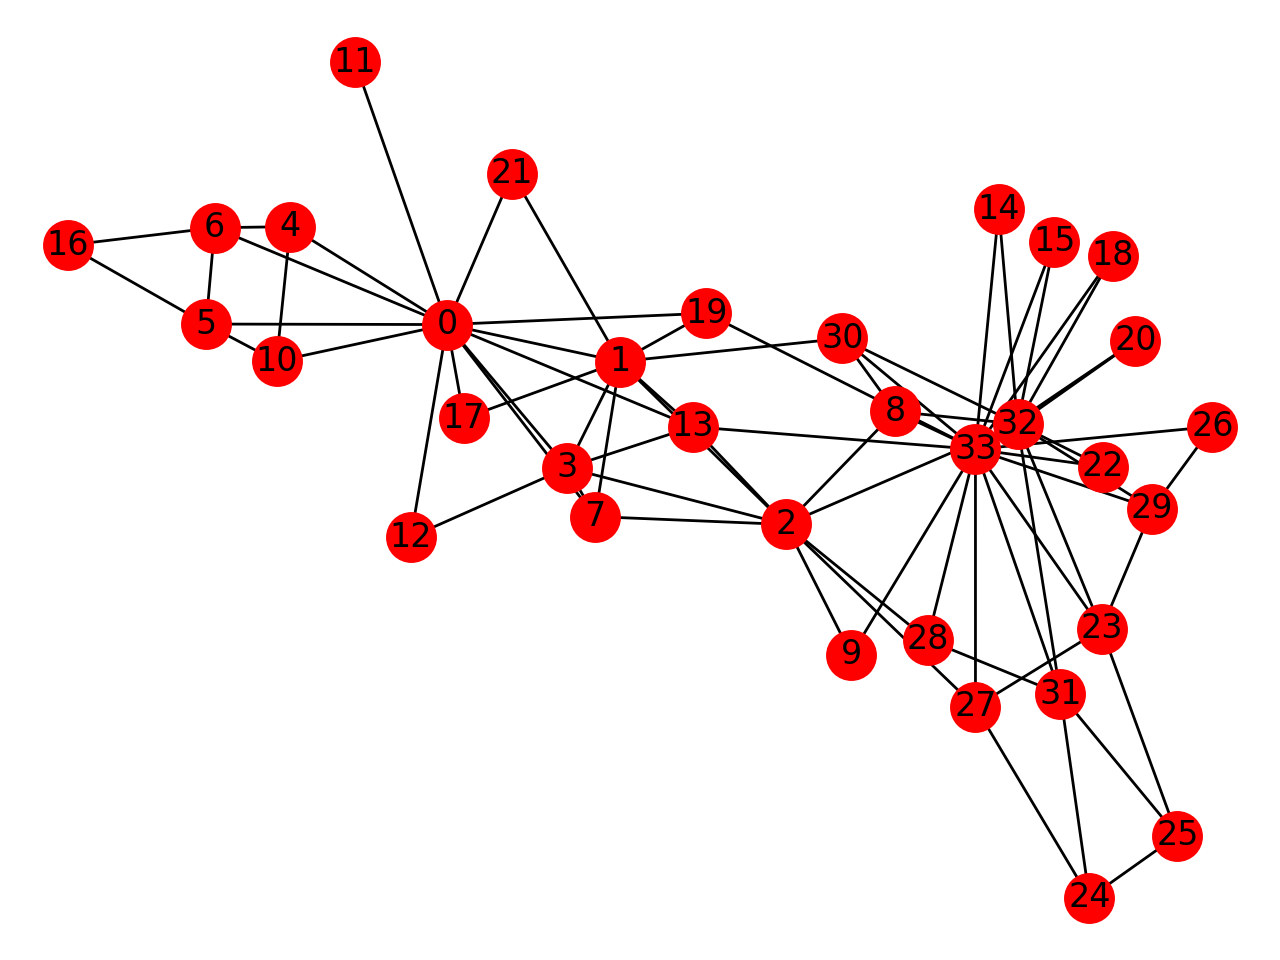
\includegraphics[width=0.8\textwidth]{F4}
      \caption{Iteration 3}
	\end{figure}
	
\begin{figure}[h]
  \centering
    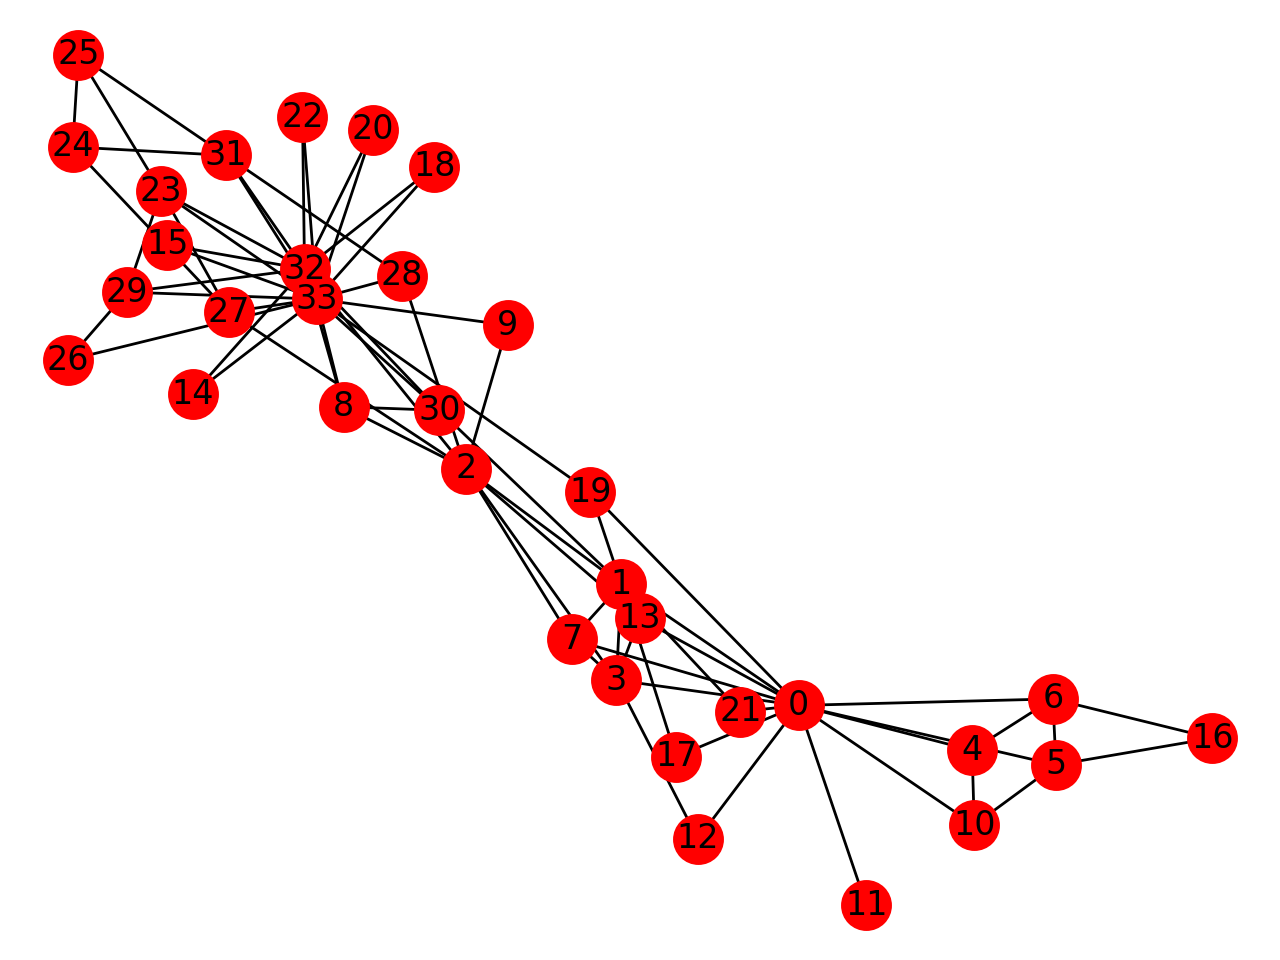
\includegraphics[width=0.8\textwidth]{F5}
      \caption{Iteration 4}
	\end{figure}	

\begin{figure}[h]
  \centering
    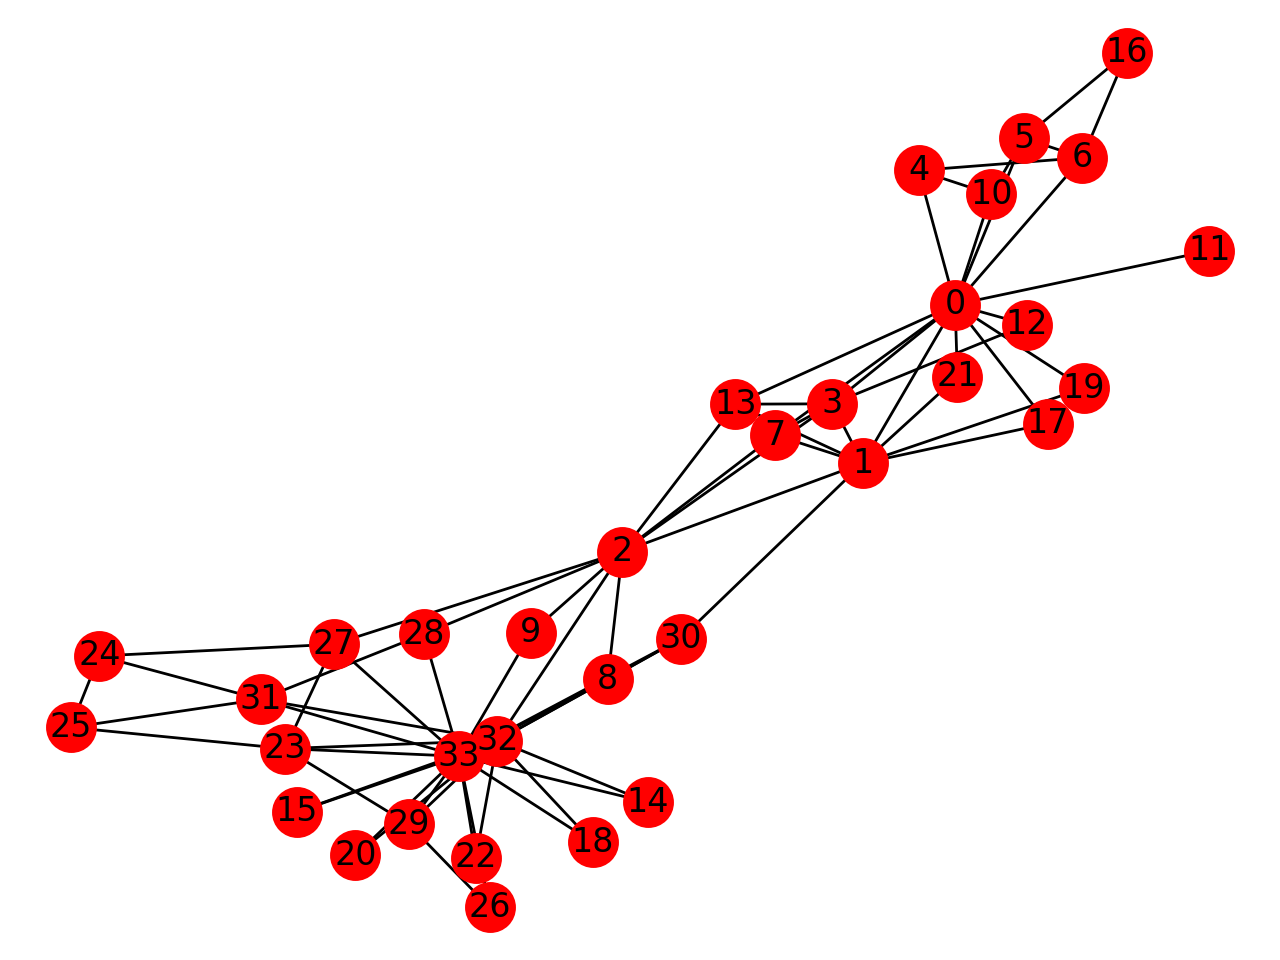
\includegraphics[width=0.8\textwidth]{F6}
      \caption{Iteration 5}
	\end{figure}
	
\begin{figure}[h]
  \centering
    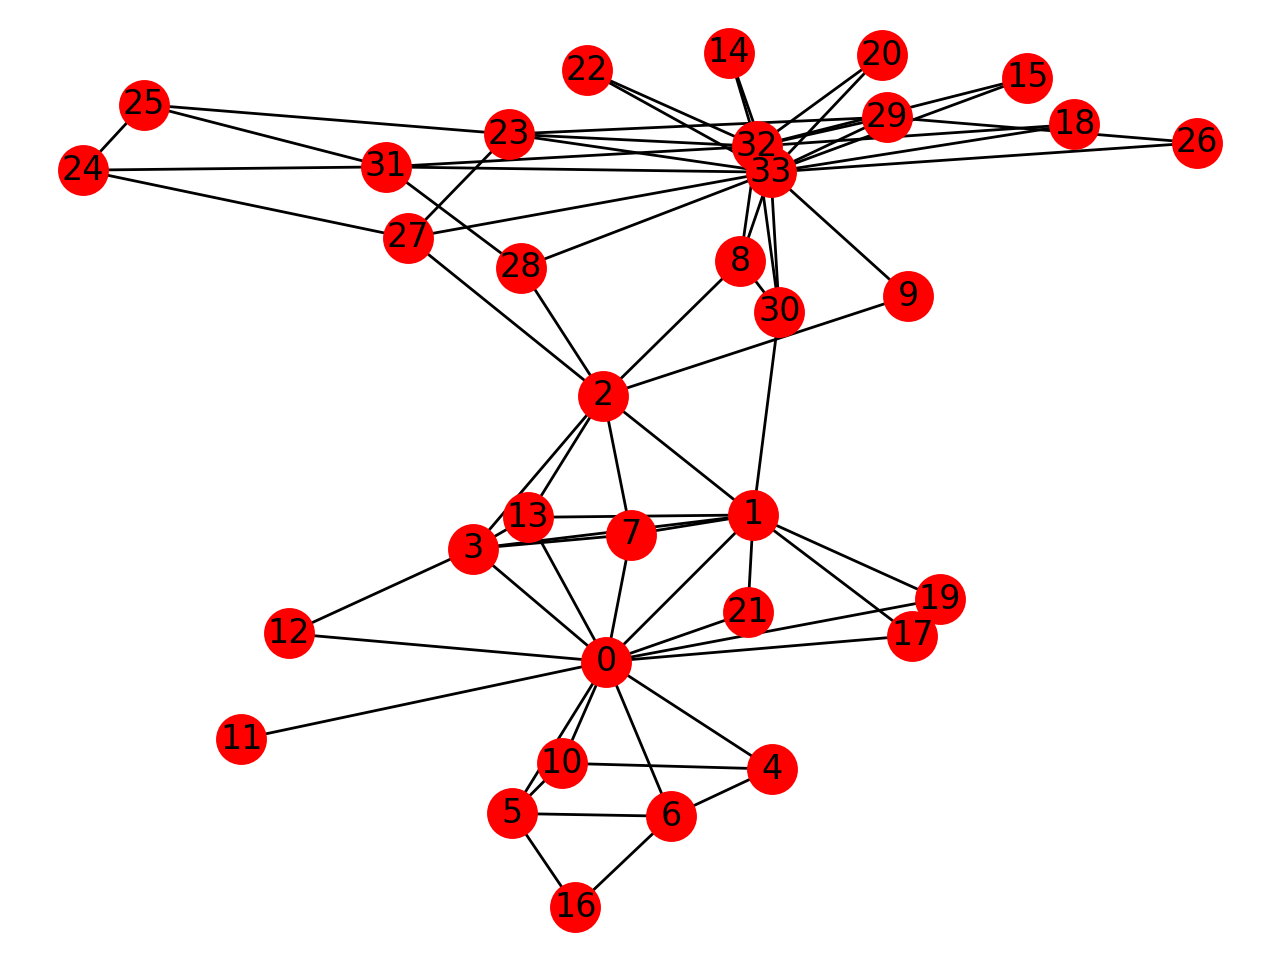
\includegraphics[width=0.8\textwidth]{F7}
      \caption{Iteration 5}
	\end{figure}
	
\begin{figure}[h]
  \centering
    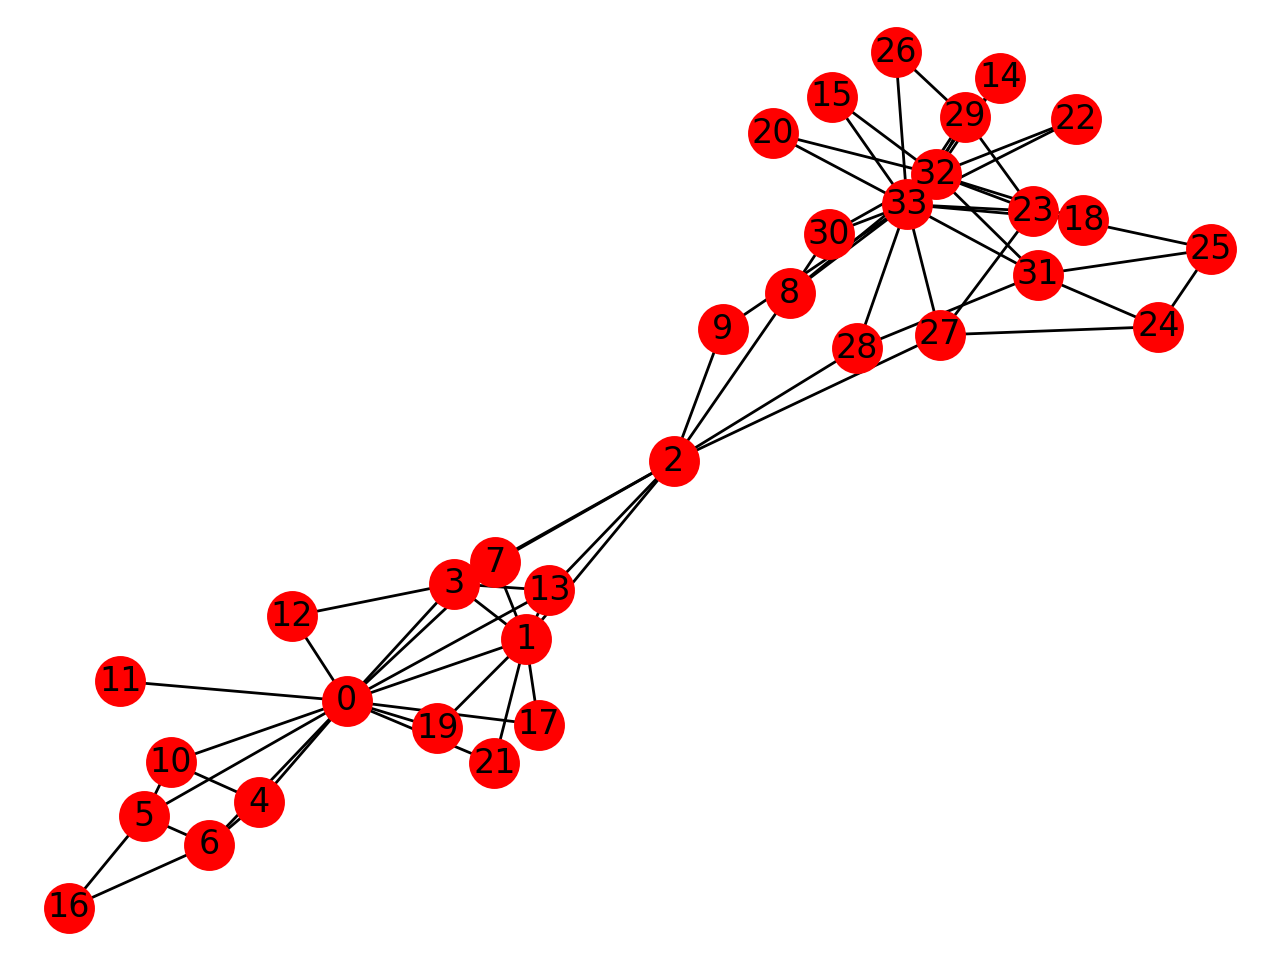
\includegraphics[width=0.8\textwidth]{F8}
      \caption{Iteration 6}
	\end{figure}
	
\begin{figure}[h]
  \centering
    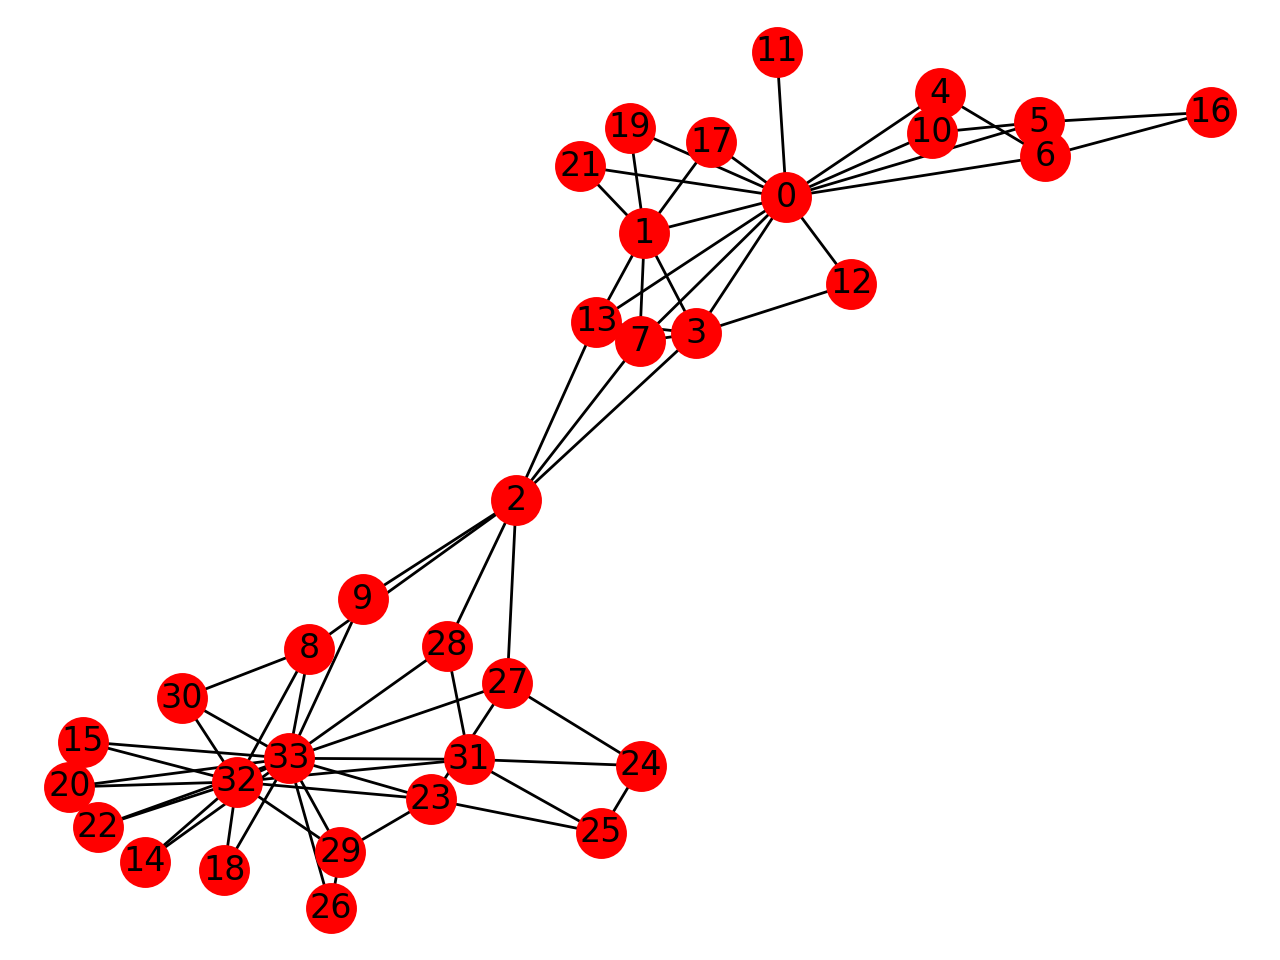
\includegraphics[width=0.8\textwidth]{F9}
      \caption{Iteration 7}
	\end{figure}
	
\begin{figure}[h]
  \centering
    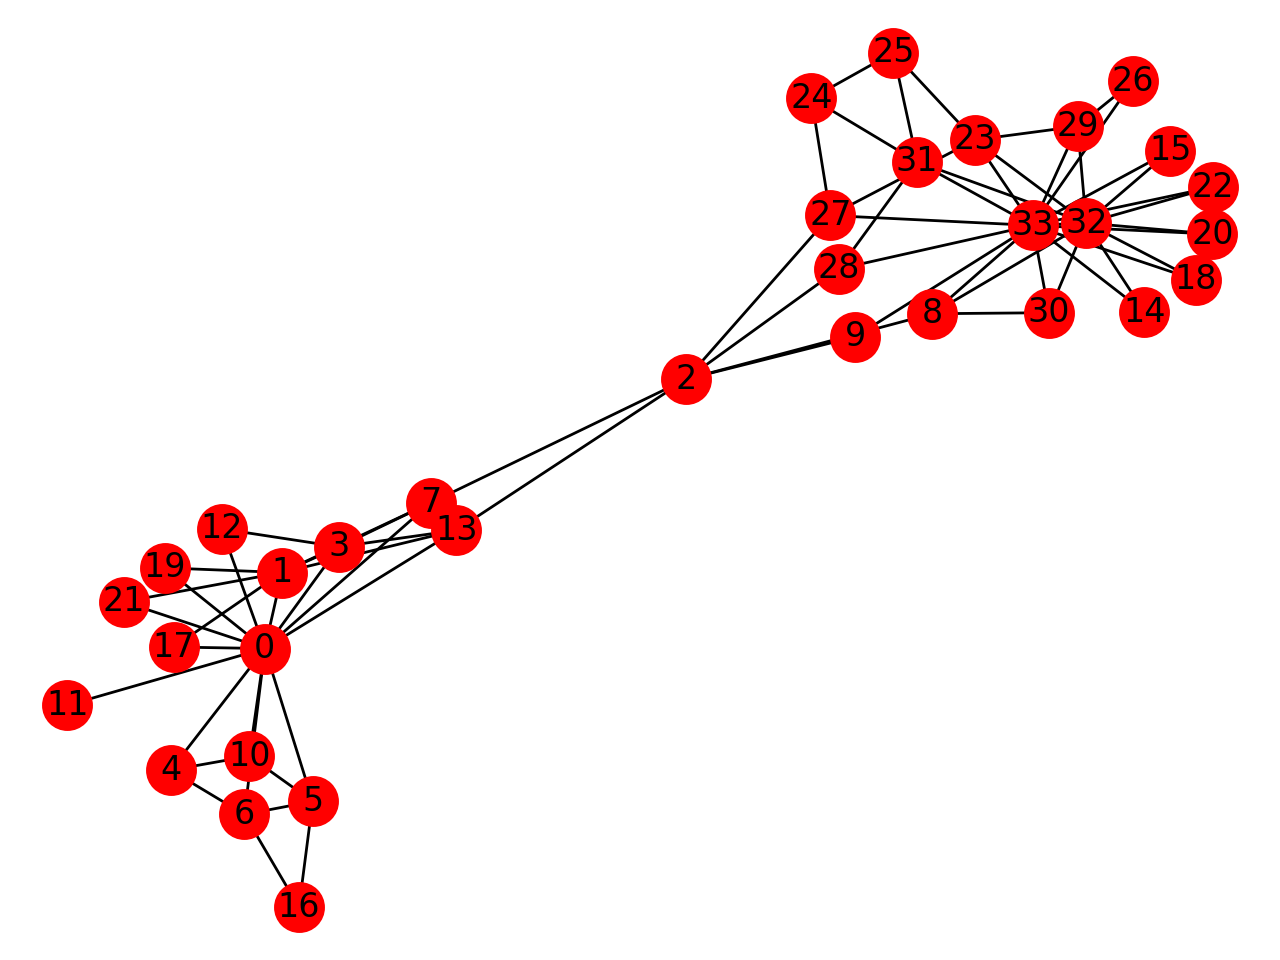
\includegraphics[width=0.8\textwidth]{F10}
      \caption{Iteration 8}
	\end{figure}
	
\begin{figure}[h]
  \centering
    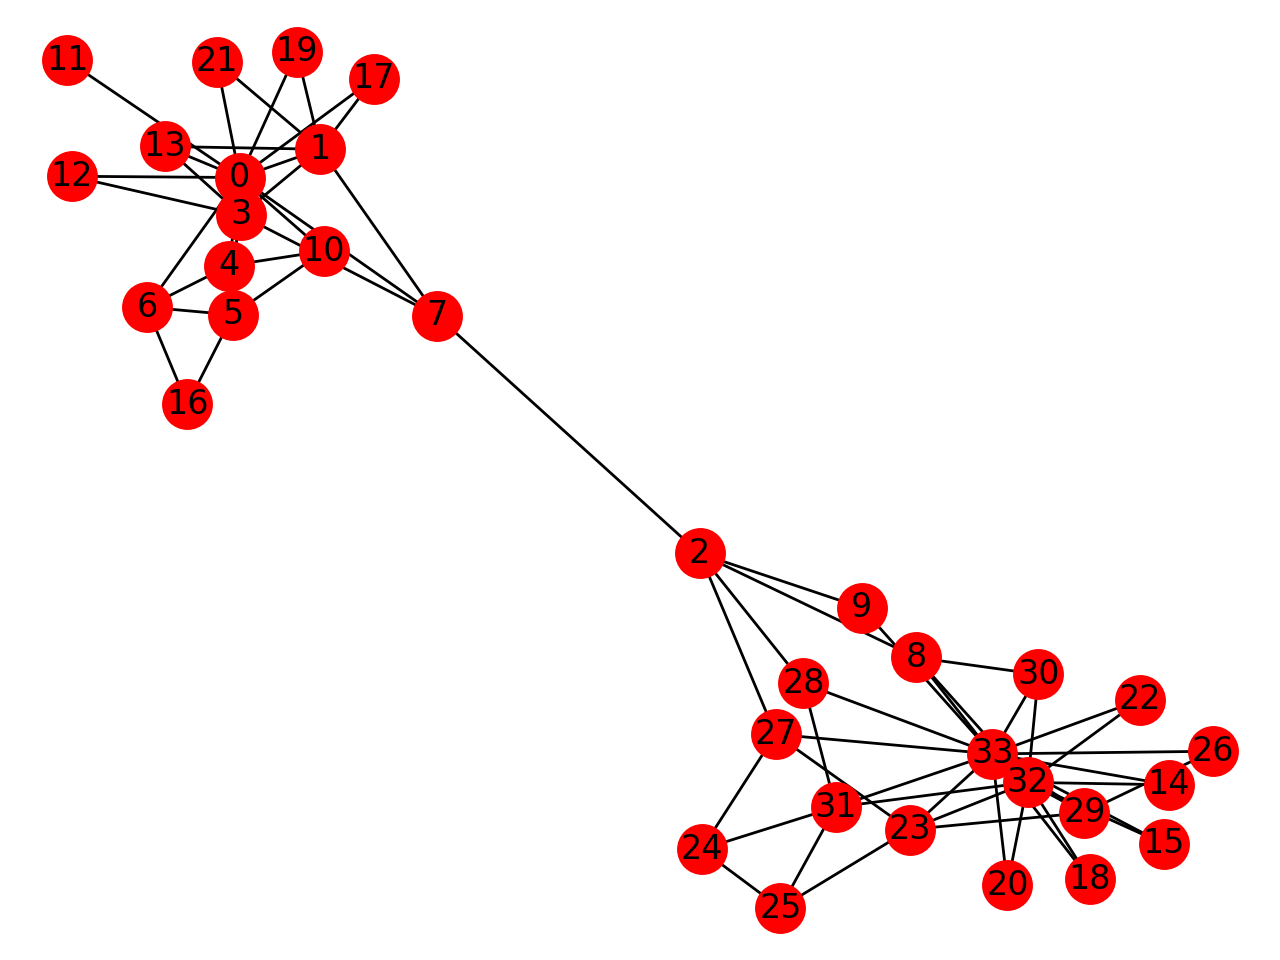
\includegraphics[width=0.8\textwidth]{F11}
      \caption{Iteration 9}
	\end{figure}
	
\begin{figure}[h]
  \centering
    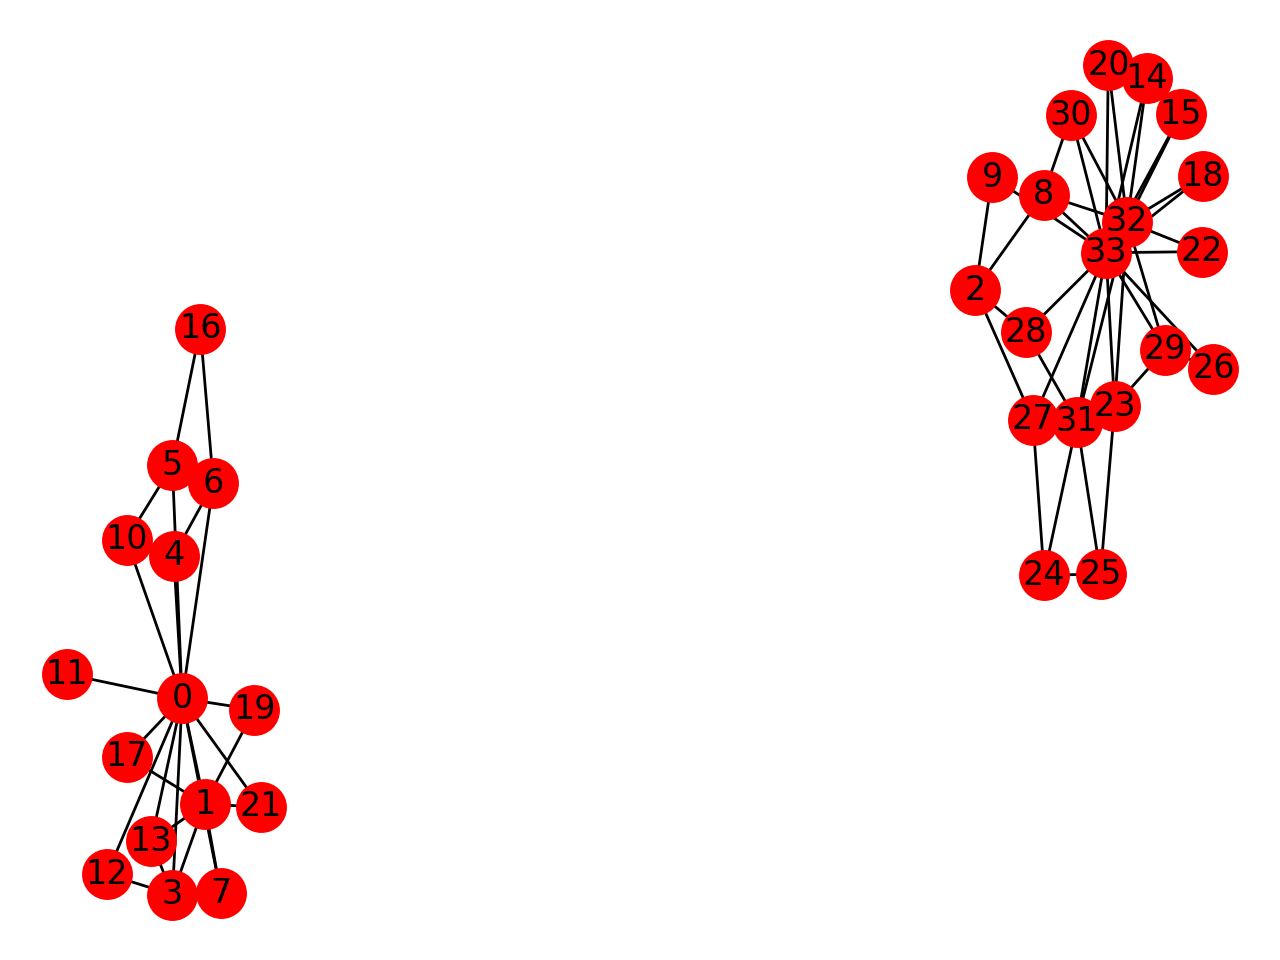
\includegraphics[width=0.8\textwidth]{F12}
      \caption{Final Segregation}
	\end{figure}
	
	
	
\end{homeworkProblem}
\clearpage
\newpage


\bibliographystyle{plain}
\bibliography{A1bibFile}

\end{document}
